%----------------------------------------------------------------------------------------
%	ARTICLE CONTENTS
%----------------------------------------------------------------------------------------

\section{Introduction}

L'objectif de ce travail est de produire un modèle statistique permettant de prévoir
les consommations des bâtiments ainsi que les rejets de gaz à effet de serre (GHG) sur
base des informations du permis d'exploitation.

Une analyse préliminaire des données ainsi que la sélection d'un modèle
adapté sont ici détaillées.
%------------------------------------------------

\section{Données disponibles}

les informations sur le set de donnée utilisé tout au long de ce travail sont exposés ici.

\subsection{généralités}

Les données sont disponibles gratuitement sur le site de la ville de seattle et
également sur la plateforme "Kaggle".

Le jeu de données contient deux fichiers :
\begin{itemize}
  \item{2015-building-energy-benchmarking.csv}
  \item{2016-building-energy-benchmarking.csv}
\end{itemize}

Les deux jeux de données contiennent essentiellement les mêmes variables mais
certaines (Par exemple : la localisation) sont encodées différemment.

\paragraph{Notes}

Les seules différences notables entre les deux jeux de données sont:
\begin{itemize}
  \item{Le jeu de 2016 contient 36 observations de plus que celui de 2015.}
  \item{Les données de 2016 n'ont pas la variable "OtherFuelUse"}
  \item{Les données de 2015 contiennent une variable "Location" contenant les
       informations suivantes}
  \begin{itemize}
    \item{City}
    \item{State}
    \item{ZipCode}
    \item{Address}
    \item{Latitude et longitude}
  \end{itemize}
  \item{Les colonnes suivantes ont été renommées}
  \begin{itemize}
    \item{Comment : comments}
    \item{GHGEmissions(MetricTonsCO2e) : TotalGHGEmissions}
    \item{GHGEmissionsIntensity(kgCO2e/ft2) : GHGEmissionsIntensity}
  \end{itemize}
\end{itemize}

%------------------------------------------------

\section{Analyse exploratoire des données}

\subsection{Travail préliminaire sur les données}

Les deux jeux de données sont uniformisés au niveau des variables
(la colonne "Location" du jeu de données de 2015 est transformée en colonnes
"Address", "ZipCode", "Latitude", "Longitude", ...) puis aggrégés pour former
un jeu unique contenant 47 variables et 6716 observations.

On a donc les variables suivantes :
  voir table \ref{tab:table-variables}

\begin{table}[p]
  \caption{liste des variables}
  \label{tab:table-variables}
\begin{tabular}{ll}
\toprule
{} &         0 \\
\midrule
OSEBuildingID                   &     int64 \\
BuildingType                    &  category \\
PrimaryPropertyType             &  category \\
PropertyName                    &    object \\
TaxParcelIdentificationNumber   &    object \\
CouncilDistrictCode             &     int64 \\
Neighborhood                    &  category \\
YearBuilt                       &     int64 \\
NumberofBuildings               &   float64 \\
NumberofFloors                  &   float64 \\
PropertyGFATotal                &     int64 \\
PropertyGFAParking              &     int64 \\
PropertyGFABuilding(s)          &     int64 \\
ListOfAllPropertyUseTypes       &    object \\
LargestPropertyUseType          &  category \\
LargestPropertyUseTypeGFA       &   float64 \\
SecondLargestPropertyUseType    &  category \\
SecondLargestPropertyUseTypeGFA &   float64 \\
ThirdLargestPropertyUseType     &  category \\
ThirdLargestPropertyUseTypeGFA  &   float64 \\
YearsENERGYSTARCertified        &    object \\
ENERGYSTARScore                 &   float64 \\
SiteEUI(kBtu/sf)                &   float64 \\
SiteEUIWN(kBtu/sf)              &   float64 \\
SourceEUI(kBtu/sf)              &   float64 \\
SourceEUIWN(kBtu/sf)            &   float64 \\
SiteEnergyUse(kBtu)             &   float64 \\
SiteEnergyUseWN(kBtu)           &   float64 \\
SteamUse(kBtu)                  &   float64 \\
Electricity(kWh)                &   float64 \\
Electricity(kBtu)               &   float64 \\
NaturalGas(therms)              &   float64 \\
NaturalGas(kBtu)                &   float64 \\
OtherFuelUse(kBtu)              &   float64 \\
TotalGHGEmissions               &   float64 \\
GHGEmissionsIntensity           &   float64 \\
DefaultData                     &    object \\
Comments                        &    object \\
ComplianceStatus                &    object \\
Outlier                         &    object \\
Latitude                        &   float64 \\
Longitude                       &   float64 \\
Address                         &    object \\
State                           &    object \\
City                            &    object \\
ZipCode                         &    object \\
\bottomrule
\end{tabular}

\end{table}

\paragraph{Suppression des observations dont la consommation est nulle}
On supprime toutes les lignes pour lesquelles la consommation du bâtiment est $\le$ 0.
Cela concerne 103 lignes sur 6716 soit 1,53 \% des données.


\subsection{Analyse des variables}

\subsubsection{Analyses univariées}

\paragraph{Usage des surfaces} On peut regarder la répartission des différents
usages de surfaces.
\begin{figure}[H]
  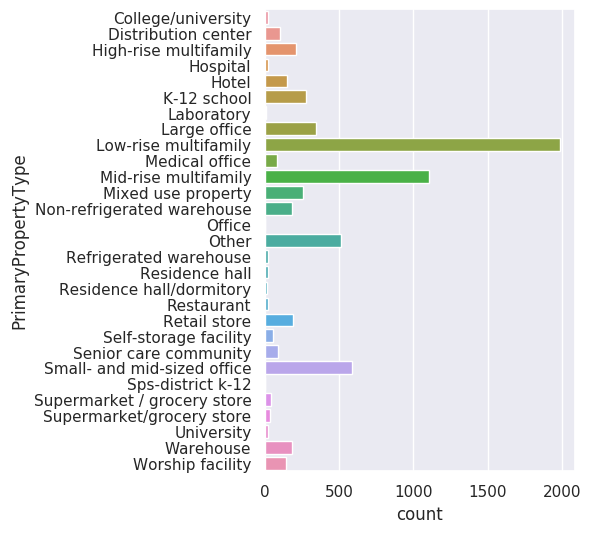
\includegraphics[width=\linewidth]{univar_primary_property_type.png}
  \caption{Principaux usages des bâtiments}
  \label{}
\end{figure}

\paragraph{Surface totale des bâtiments} On regarde la distribution des valeurs
de GFA (gross floor area.)
\begin{figure}[H]
  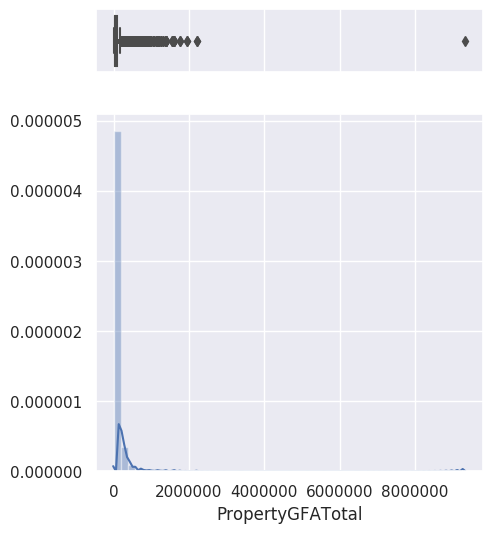
\includegraphics[width=\linewidth]{univar_property_gfa_total.png}
  \caption{Principaux usages des bâtiments}
  \label{}
\end{figure}



\subsubsection{Analyses bivariées}

On cherche quelles sont les variables corrélées avec la consommation d'énergie
du bâtiment.

\paragraph{Lien entre la surface du bâtiment et la consommation}

\begin{figure}[H]
  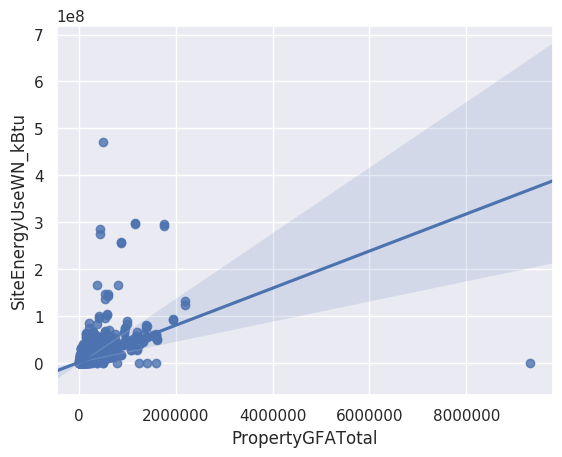
\includegraphics[width=\linewidth]{bivar_gfa_energy.png}
  \caption{Régression linéaire entre la surface du bâtiment (TotalGFA) et la
  consommation}
  \label{}
\end{figure}

\begin{figure}[H]
  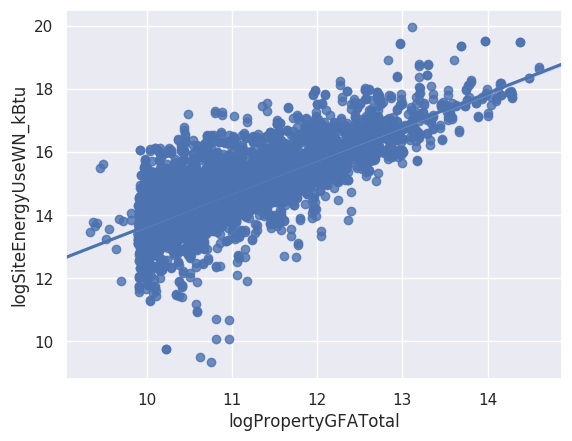
\includegraphics[width=\linewidth]{bivar_gfa_energy_log.png}
  \caption{Régression linéaire entre la surface du bâtiment (TotalGFA) et la
  consommation avec passage en log}
  \label{}
\end{figure}

On observe une corrélation entre les variables.

\begin{table*}[p]
\centering
\begin{tabular}{@{}llll@{}}
\toprule
\multicolumn{4}{c}{OLS Regression Results}                             \\ \midrule
Dep. Variable:    & PropertyGFATotal & R-squared:          & 0.244     \\
Model:            & OLS              & Adj. R-squared:     & 0.244     \\
Method:           & Least Squares    & F-statistic:        & 2166.     \\
Date:             & Mon, 02 Mar 2020 & Prob (F-statistic): & 0.00      \\
Time:             & 08:12:49         & Log-Likelihood:     & -89924.   \\
No. Observations: & 6700             & AIC:                & 1.799e+05 \\
Df Residuals:     & 6698             & BIC:                & 1.799e+05 \\
Df Model:         & 1                &                     &           \\
Covariance Type:  & nonrobust        &                     &           \\ \bottomrule
\end{tabular}
\end{table*}

\begin{table*}[p]
  \centering
\begin{tabular}{@{}lllllll@{}}
\toprule
coef                  & std err   & t        & P\textgreater{}|t| & {[}0.025 & 0.975{]} &          \\ \midrule
Intercept             & 5.791e+04 & 1497.499 & 38.669             & 0.000    & 5.5e+04  & 6.08e+04 \\
SiteEnergyUseWN\_kBtu & 0.0062    & 9.35e-05 & 66.432             & 0.000    & 0.006    & 0.006    \\ \bottomrule
\end{tabular}
\end{table*}

\begin{table*}[p]
  \centering
\begin{tabular}{@{}llll@{}}
\toprule
\multicolumn{4}{c}{OLS Regression Results}                                \\ \midrule
Dep. Variable:    & logPropertyGFATotal & R-squared:          & 0.622     \\
Model:            & OLS                 & Adj. R-squared:     & 0.622     \\
Method:           & Least Squares       & F-statistic:        & 1.070e+04 \\
Date:             & Thu, 27 Feb 2020    & Prob (F-statistic): & 0.00      \\
Time:             & 17:30:22            & Log-Likelihood:     & -5037.7   \\
No. Observations: & 6512                & AIC:                & 1.008e+04 \\
Df Residuals:     & 6510                & BIC:                & 1.009e+04 \\
Df Model:         & 1                   &                     &           \\
Covariance Type:  & nonrobust           &                     &           \\ \bottomrule
\end{tabular}
\end{table*}

\begin{table*}[p]
  \centering
\begin{tabular}{@{}lllllll@{}}
\toprule
coef                     & std err & t     & P\textgreater{}|t| & {[}0.025 & 0.975{]} &       \\ \midrule
Intercept                & 2.2812  & 0.084 & 27.228             & 0.000    & 2.117    & 2.445 \\
logSiteEnergyUseWN\_kBtu & 0.5906  & 0.006 & 103.447            & 0.000    & 0.579    & 0.602 \\ \bottomrule
\end{tabular}
\end{table*}


\paragraph{Lien entre le type d'utilisation et la consommation}
On peut regarder si le type d'utilisation des surfaces impact la consommation du bâtiment.
On réalise donc une analyse de type "ANOVA" \cite{rutherford2001introducing}(analyse of variance) pour déterminer
si l'usage (donnée catégorielle) impact la consommation (ici consommation au mètre carré\footnote{Les données provenant des US, les données sont exprimées dans les unités US (kBtu/sf)}). On peut ensuite poursuivre l'analyse par
un test des paires HSD de Tukey \cite{abdi2020} (Pour déterminer quel type d'usage impact la moyenne.)

On remarque alors qu'un grand nombre d'usage type n'ont pas d'impact sur la moyenne.


\begin{figure*}
  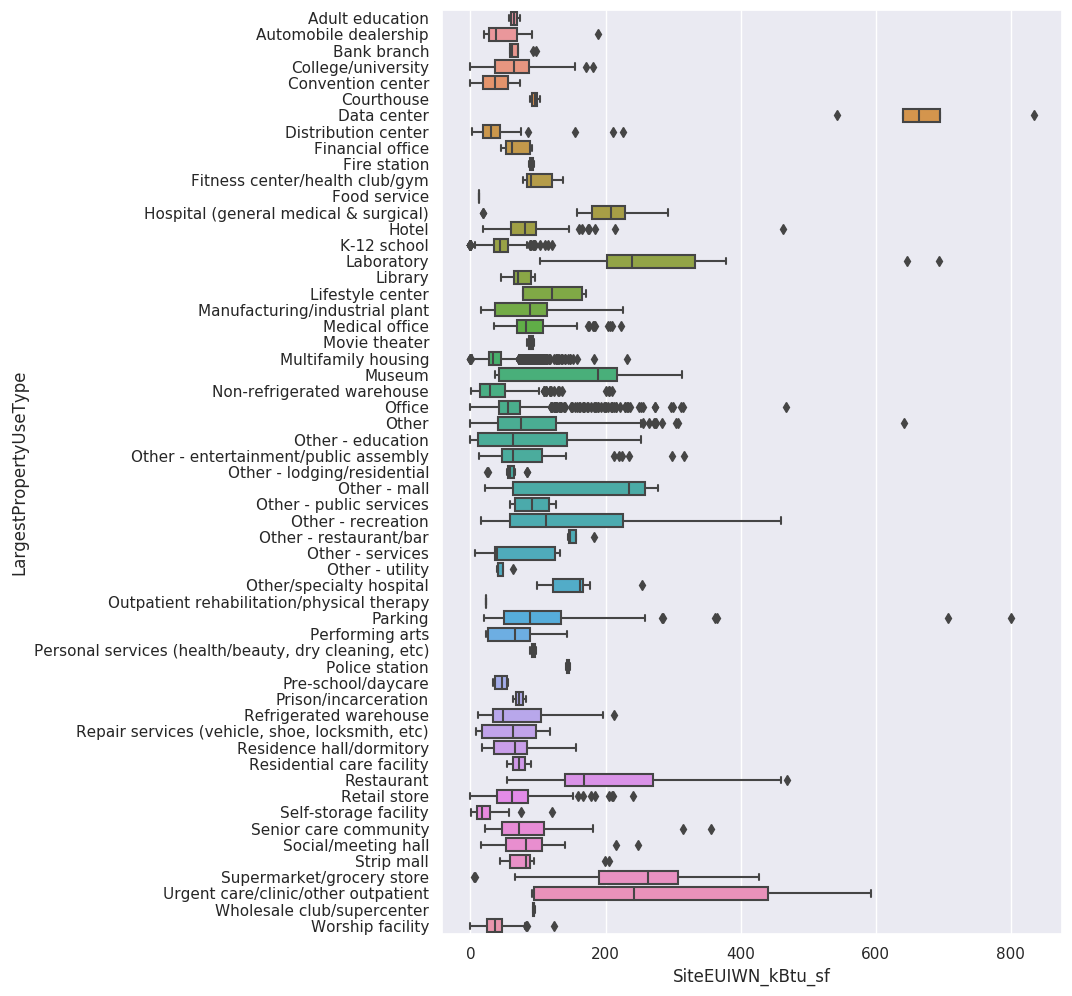
\includegraphics[width=\linewidth]{ANOVA_1.png}
  \caption{}
  \label{}
\end{figure*}
\begin{figure*}
  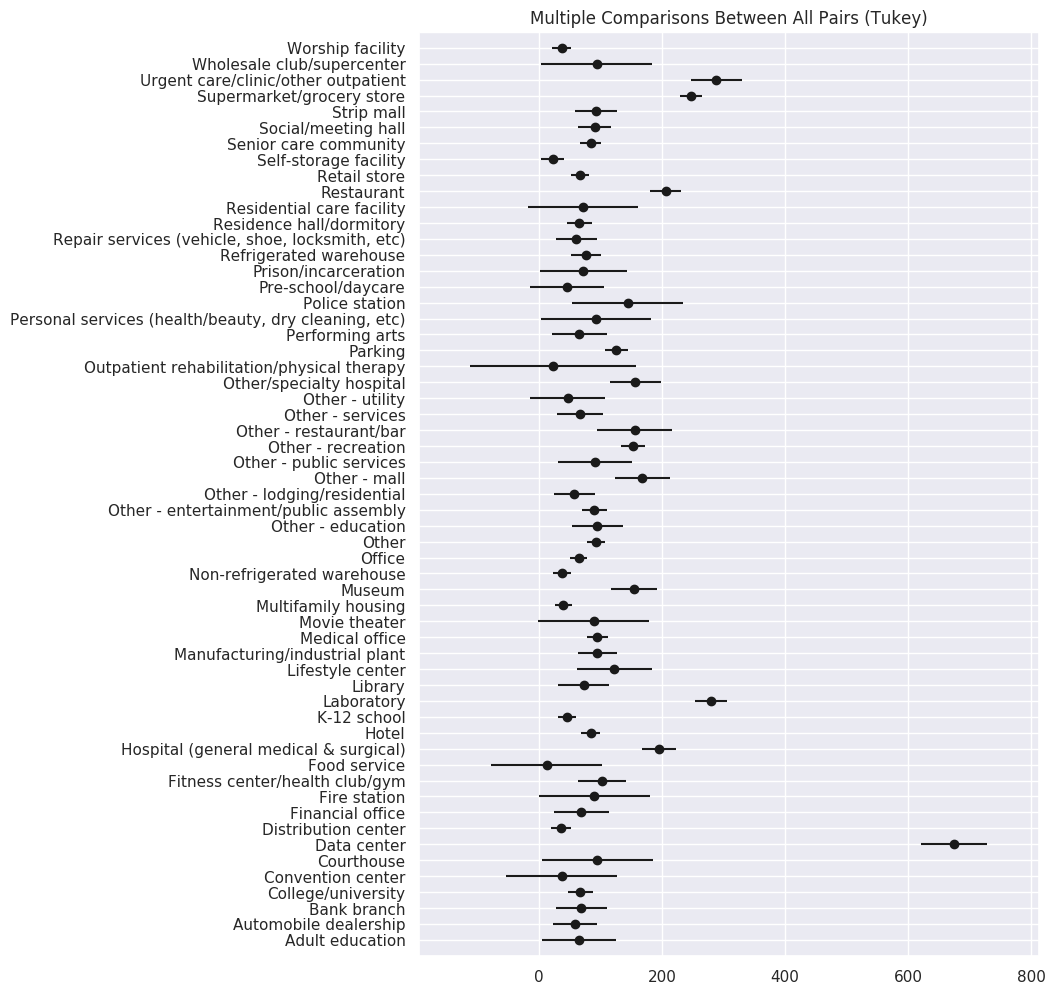
\includegraphics[width=\linewidth]{TukeyHSD_1.png}
  \caption{}
  \label{}
\end{figure*}




\subsubsection{Feature engineering}

Les données sont ré-encodées différemment pour servir d'entrée au modèle



%------------------------------------------------

\section{Modèle}


\subsection{Données d'entrée (input)}

On utilise les données préalablement ré-encodées comme entrée du modèle.
On a donc 65 variables d'entrée pour le modèle (64 usages type des surfaces ainsi
que la surface totale.).
Les 64 premières colonnes sont donc des flotants (float64) compris entre 0 et 1.
La 65\up{ème} colonne contient les surfaces totale (TotalGFA) cette dernière
subit une transformation logarithmique lors de l'entrainement du modèle.

\subsection{Données de sortie (output)}

Dans un premier temps, on se focalise uniquement sur la consommation énergétique
des bâtiments et non sur la production de GHG (Les GHG sont traités plus loin
dans le document).

\subsection{Sélection du modèle}

Pour sélectionner un modèle, on entraîne successivement les modèles de
régression suivant:
\begin{itemize}
  \item LinearRegression (Régression linéaire simple)
  \item Régression linéaire avec régularisation.
  \begin{itemize}
    \item Ridge \cite{Marquardt1975}
    \item Lasso \cite{tibshirani96regression}
    \item ElasticNet
  \end{itemize}
  \item Régression non linéaire.
  \begin{itemize}
    \item Support Vector Machine (support vector regression SVR)
    \item Stochastic gradient descent (SGDRegressor)
    \item Nearest neighbors (KNeighborsRegressor)
    \item Arbres de décision (DecisionTreeRegressor)
  \end{itemize}
  \item Méthode d'ensemble
  \begin{itemize}
    \item RandomForestRegressor
    \item GradientBoostingRegressor
  \end{itemize}
  \item Réseau de neurones artificiels: Multilayer perceptron (MLPRegressor)
\end{itemize}

On peut alors comparer les résultats obtenus sur ces modèles.
\begin{table}[H]
  \begin{tabular}{lrr}
\toprule
{} &     score &  score train \\
\midrule
LinearRegression          &  0.749299 &     0.809332 \\
Ridge                     &  0.749725 &     0.774537 \\
Lasso                     &  0.756173 &     0.788543 \\
Elastic-Net               &  0.752422 &     0.778566 \\
SGDRegressor              &  0.536248 &     0.488317 \\
KNNRegressor              &  0.648070 &     0.774813 \\
DecisionTreeRegressor     &  0.828981 &     0.999986 \\
GradientBoostingRegressor &  0.701887 &     0.770610 \\
RandomForestRegressor     &  0.747167 &     0.912144 \\
SVR                       &  0.743089 &     0.870307 \\
MLP                       &  0.778817 &     0.797352 \\
\bottomrule
\end{tabular}

  \caption{Scores obtenus avec paramètres par défaut}
  \label{}
\end{table}

Hormis la régression linéaire simple, l'ensemble des modèles utilisés comportent
des hyperparamètres\footnote{On fait la distinction ici entre les paramètres
qui sont optimisés au sein du modèle et les paramètres externe au modèles appelés
hyperparamètres.} à optimiser.
Pour une comparaison des modèles en bon et dû forme, il est possible d'optimiser
les hyperparamètres de manière récursive et de comparer les modèles optimisés.
\footnote{Certain modèle demande un temps calcul non négligeable et prennent donc
du temps à entrainer, à ce stade, les modèles sont donc grossièrement optimisés
pour comparaison.}

\begin{figure}[H]
  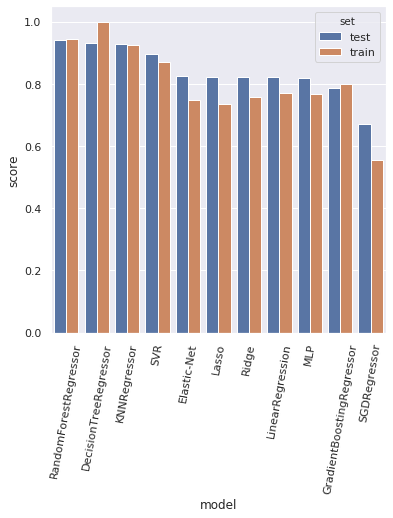
\includegraphics[width=\linewidth]{models_scores.png}
  \caption{scores obtenus pour les modèles de régression}
  \label{}
\end{figure}

\subsection{Algorithme sélectionné}

\subsubsection{RandomForestRegressor}

\paragraph{Avantages} Meilleure généralisation
(Le modèle donne des résultats très similaires sur les données d'entrainement et
sur les donnnées de test. ).

\paragraph{Points faibles}

\subsubsection{DecisionTreeRegressor}

\paragraph{Avantages}

\paragraph{Points faibles}

\subsubsection{Modèle retenu}




\subsection{Entrainement du modèle}


%------------------------------------------------

\section{Résultats}


%------------------------------------------------

\section{Conclusion}


%------------------------------------------------
